\section{Materials and methods}

\subsection{Molecular docking}
See comments in source

\begin{figure}[h]
\centering
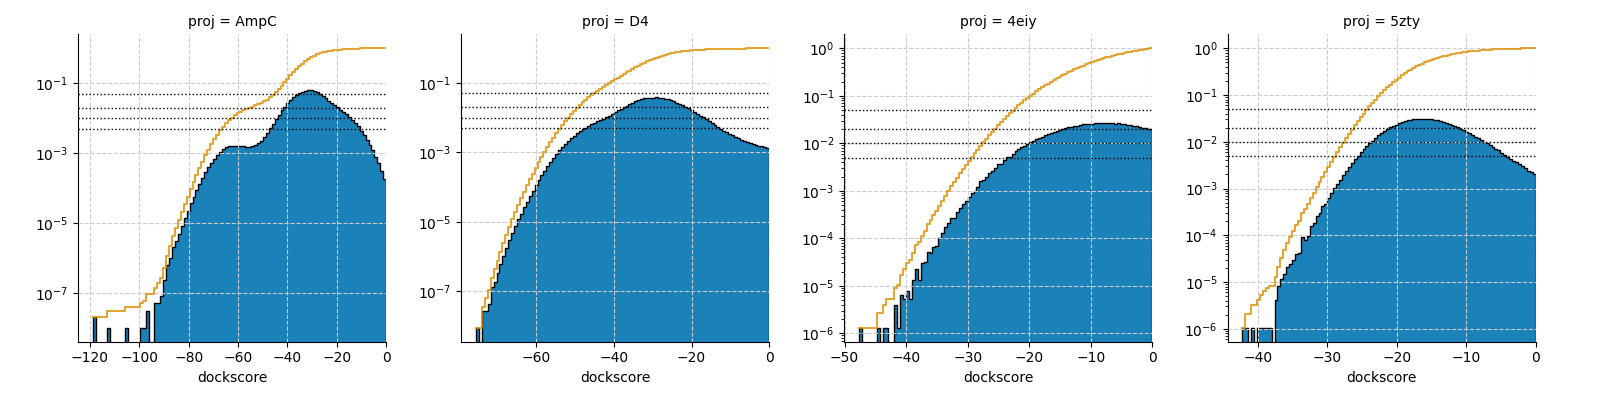
\includegraphics[width=0.8\textwidth]{figures/Figure_1.png}
\caption{distributions of scores for datasets used in the study. Histogram (blue) shows log-scale score distribution, while plot (orange) shows cumulative distribution of scores. Horizontal line (black) shows cutoff for top-1\% of scores.}
\label{fig:fig_1}
\end{figure}

% Fig 1: description of all datasets used in the paper
% 	- number of ligands
% 	- score distributions
% 	- ? structure

\subsection{Prediction of docking scores} \label{subsec:prediction}
See comments in source


% how we did machine learning
% ? Fig 2: machine learning pipelines
% 	- A: cross-validation scheme for "best model" figure
% 	- B: cross-validation scheme for iterations
% 	- what "iterations" mean & their different regimes (from diploma)

